\chapter{Optimal Portfolio Allocation}
\label{chpr:markowitz}

In this chapter we will explore what the optimal allocation is for our portfolio of assets. We will study the \textit{efficient frontier} using two different risk measures, volatility and expected shortfall. In all our analyses, we will be comparing the effects that including Bitcoin in our portfolio has on the optimal allocation.


\section{Markowitz Mean-Variance Portfolio Optimization}

Modern Portfolio Theory (MPT) is a mathematical framework for creating a portfolio of asset by maximizing the expected return for a given level of risk or by minizing the risk while maintaining the same expected gain. 
Before the article \cite{MARKOWITZ1952} by Harry Markowitz in 1952, the concept of \textit{diversification} (the old warning \textit{not to put all your eggs in one basket}) was only driven by the experience of how markets behave.
Moreover, investors used to base their decisions on expected return alone and thus when given a choice between two assets with different expected returns, they would put all their money on the top performing one.

With his article, that would later grant him the Nobel Prize in Economics, Markowitz introduced a more rigorous and mathematically sound framework to assembly a portfolio of assets. His key insight is that an asset's return and risk risk should not be assessed by itself, but rather by how it affects the overall portfolio risk and return.
To do so, the \textit{variance} is used as a proxy for risk. Hence the name \textit{mean-variance } analysis that is often used as a substitute for MPT.

\bigskip
Let's introduce the assumption underlying the MPT:
\begin{enumerate}
	\item Investors are \textit{risk averse}: they will always choose the less risky asset, when two assets offer the same return.  At the same time, an investor wanting a higher return has to be willing to accept a higher risk.
	This equally holds for portfolios as a whole: given two portfolio with the different risk profiles, he will choose the less risky in case of same return and the most remunerating in case of same risk.
	\item Portfolio return is the weighted sum of the single assets' returns: in general $\mathbb{E}[R_{ptf}] = \sum_{i=1}^{N} w_i \mathbb{E}[R_i]$.
	\item Portfolio variance is a function of both the assets variances and their correlations: $V_{ptf} = \sum_{i=1}^{N} w_i \sigma_i^2 + \sum_{i=1}^{N}\sum_{j\neq i , j=1}^{N} w_i w_j \rho_{i,j}\sigma_i\sigma_j$
\end{enumerate}

Items 2 and 3 above can be more compactly stated using matrix notation, which will come in handy later on in our analysis:
\begin{equation}
\label{eq:ptf_return}
r_{ptf}(\mathbf{w}) = \mathbf{w}^T \mathbf{r}
\end{equation}
\begin{equation}
\label{eq:sigma_ptf}
	\sigma^2_{ptf}(\mathbf{w}) =  \mathbf{w}^T \Sigma \mathbf{w}
\end{equation}

where we have the weights vector $\mathbf{w} = [w_1, w_2, ... , w_N]^T$ , $\mathbf{r} = [r_1, r_2, ... , r_N]^T$, using the shorthand $r_i = \mathbb{E}[R_i]$ and finally $\Sigma$ is the $NxN$ covariance matrix of the assets.

\bigskip

We can now state the \textit{optimization problem} involving the minimization of the portfolio risk for a specified expected portfolio return in terms of the variable we have just introduced.

\begin{subequations}
	\label{eq:markowitz_opt}
	\begin{align}
%	\label{eq:mark_min}
	&\!\min_{\mathbf{w}\in \mathbb{R}^{N}}     &    & \sigma^2_{ptf}(\mathbf{w}) \\
%	\label{eq:mark_weights}
	& \text{subject to}   &   & \mathbf{e}^T\mathbf{w} = 1 ,\\
%	\label{eq:mark_return}
	&                 &       & \mathbf{r}^T\mathbf{w} = r_{target},\label{eq:constraint2} \\
%	\label{eq:mark_noshort}
	&		   &      & w_{i} \geq 0, \text{for} \: i = 1\dots N. 
	\end{align}
\end{subequations}

where \textbf{e} indicates a vector of ones and the first constraint makes sure that the sum of the weights always equals to one. This is to represent a portfolio in which all the money available is allocated in the assets we are taking into consideration.
The second constraint ensures that the portfolio allocation $\mathbf{w}$ produces the target expected return $r_{target}$.
Finally, the last constraint is in fact optional and is only used to exclude the possibility to go short on any asset.

The optimization problem in \eqref{eq:markowitz_opt} has a quadratic objective function given by \eqref{eq:sigma_ptf} and only has linear constraints\footnote{The last positivity constraint can be easily expressed in matrix form by writing $ \mathbf{I}_N\mathbf{w} \geq \mathbf{0}_N$ where $\mathbf{I}_N$ is the identity matrix of order $N$ and $\mathbf{0}_N$ is N-dimensional vector of zeros.}. Thanks to this property, the optimization can be carried out numerically by any of the quadratic/linear optimizers that are available for most programming languages.

As we are going to explain in the following sections, we will be mainly focusing on the case where there is no short selling, as indeed so far there are no instruments on the market that allow an investor to go short on Bitcoin and our analysis shows that the main diversification advantage comes from including Bitcoin in our portfolio. Allowing short-selling improves our diversification capability only so slightly.

\section{Efficient Frontier}
It is interesting to study the set of optimal allocation as a whole, rather than simply focus on one target return and minimizing the portfolio risk.
To do so, we can consider a set of target returns and compute for each of them the respective minimum variance. We thus get a set of pairs $(\sigma^2, r)$ that represents the best allocation in terms of the minimum risk.

We can thus plot those pairs on an X-Y graph and obtain a curve, the \textit{portfolio frontier}, that intrinsically represents our portfolio of $N$ assets.
As a usual practice in finance, we will be plotting on the X-axis the volatility $\sigma$ instead of the variance $\sigma^2$.

\begin{figure}
	\centering
	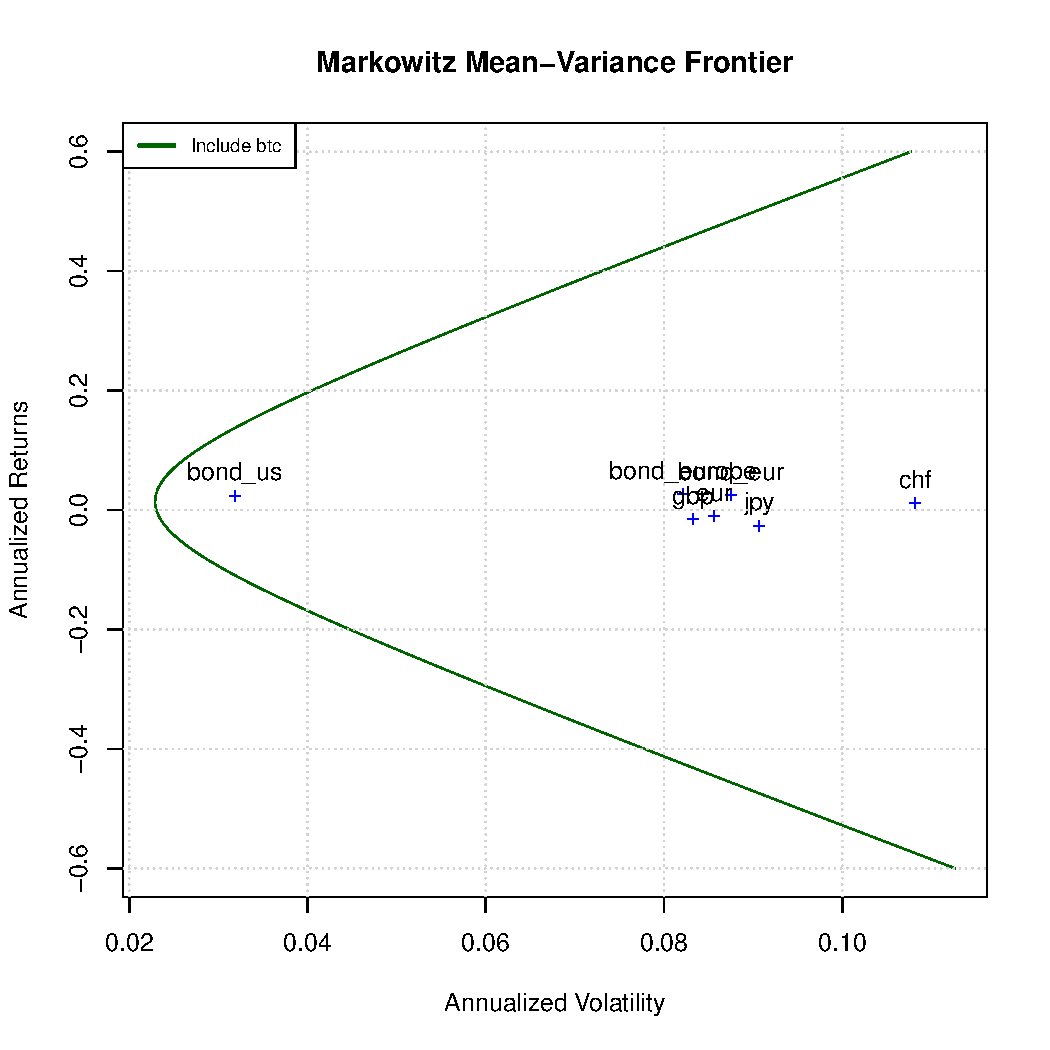
\includegraphics[width=0.6\textwidth]{Images/full_frontier.pdf}
	\caption{The Markowitz Mean-Variance frontier obtained from our portfolio of assets, that includes Bitcoin and allows short-selling.}
	\label{fig:full_frontier}
\end{figure}

In Figure \ref{fig:full_frontier} we can see what the portfolio frontier looks like for our portfolio of assets. 
It is interesting to notice how the curve divides the plane in two region: the area to the left of the line includes all those pairs $(\sigma, r)$ that are not attainable with our assets, since they have a volatility that is too low for that level of expected return. On the other hand, the region to the right of the portfolio frontier is made of all the pairs that are possible to obtain with a specific allocation $\mathbf{w}$ but that will never be chosen by an investor: moving to the left on the same level of return we eventually reach a point on the frontier. The portfolio represented by this point will dominate the one we started from in terms of risk, so it will always be a better choice.

We can proceed with the same argument arguing in terms of best return for a given level of risk: we can thus introduce the \textit{efficient} frontier. For every level of volatility that has two corresponding points on the portfolio frontier, only the one with the higher expected return will be chosen by an investor in our reference framework: hence only the top half of the curve (from the vertex and up) will form the \textit{efficient portfolio frontier}.

As a summary, let us keep in mind that any point in the volatility-expected return plane \textit{dominates} all the other portfolio allocations that are represented by points situated below and to the right of it. Conversely, that same point will be dominated by all other allocations above and to the left of it. 


\subsection{Efficient Frontier with and without Bitcoin}

Let us now study how including Bitcoin in our portfolio of assets can help increase the diversification and obtain a higher (expected) return with a lower risk.

In Figure \ref{fig:efficient_frontier_comparison} we have plotted the efficient Markowitz frontier in all possible cases: including and excluding Bitcoin while allowing short-selling, and the same curves when short-selling is not allowed.

Comparing the two green lines, we can clearly see that the exclusion of short-selling does not penalize our efficient allocation by much. The same can be stated for the red and orange curves, which represent our portfolio when excluding the digital asset.
Thus, given our particular set of assets, allowing for short-selling does very little to improve the diversification of our portfolio.

Let us now take a look of what happens when we include Bitcoin in the reference portfolio: we get a significant improvement in the expected return when considering a certain level of risk. Equivalently, for the same level of return we have a noticeable decrease in the volatility of our portfolio.

*****add numerical example, e.g. at vol=0.035 we double the return*****

\begin{figure}
	\centering
	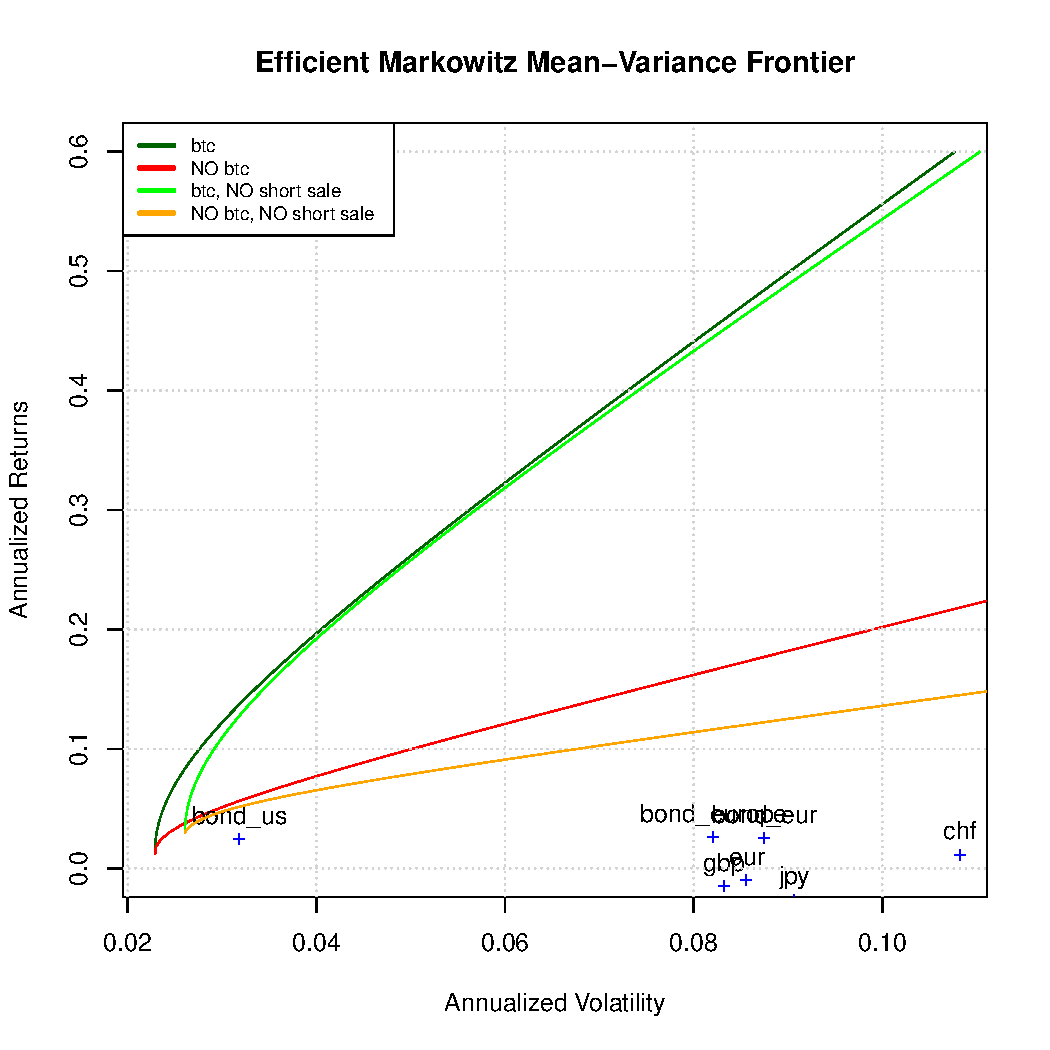
\includegraphics[width=0.6\textwidth]{Images/efficient_frontier.pdf}
	\caption{The \textit{Efficient} Markowitz Mean-Variance frontier obtained from our portfolio of assets, both including and excluding Bitcoin and with short-selling or not.}
	\label{fig:efficient_frontier_comparison}
\end{figure}





